\chapter{The {\tt Mosaic} Module}\label{ch:mosaic-module}

The \verb#Mosaic# module provides a number of tools for assembling and
generating image mosaics, i.e. large images that are composed of a
number of smaller images.  The applications of this module include
panoramic imaging and aerial/satellite image processing.  There are 
three major facilities provided at this time: compositing many images 
together, using multi-band blending to seamlessly merge overlapping 
images, and generating on-disk image quad-trees to efficiently store 
very large images.

Note that the facilities described in this chapter are currently under
active development, and there may be some API changes in future
releases as new capabilities are added.

\section{{\tt ImageComposite} and Multi-Band Blending}\label{sec:imagecomposite}

The \verb#ImageComposite# template class provides the ability to
composite any number of source images together at arbitrary pixel
offsets.  It was originally designed for assembling tiled panoramas or
aerial/satellite images that have been transformed into a common
coordinate system, though it can be used for many other things as
well.

The interface is fairly simple.  Just like ordinary Vision Workbench
images, an \verb#ImageComposite# is templatized on its pixel type.  In
most cases you will want to use a pixel type that has an alpha
channel, and if you want to perform image blending then the pixel type
must be floating-point, so the most common pixel type is
\verb#PixelRGBA<float32>#.  You can then configure whether you would
like to use multi-band blending to merge your images or if you would
simply like them overlayed by using the \verb#set_draft_mode()#
method.  It takes a single argument which should be \verb#true# if you
simply want to overlay the images and \verb#fales# if you want to use
the blender.  Blending is a significantly more expensive operation.
If your images are simply tiles and do not overlap then draft mode is
probably what you want.  In blending mode you also have the option of
asking the blender to attempt to fill in any missing
(i.e. transparent) data in the composite using information from the
neighboring pixels.  You can enable or disable this behavior by
calling the the \verb#set_fill_holes()# method.

Once you have created the composite object, you add source images to
it using the \verb#insert()# method, which takes three arguments: the
image you are adding, and the $x$ and $y$ pixel offset of that image
within the composite.  The \verb#ImageComposite# does not store a copy
of your image.  Instead, it only stores a reference to it in the form
of an \verb#ImageViewRef# object.  This means that you can easily do
things like create a composite of images that could not all fit in
memory simultaneously, e.g. by passing in \verb#DiskImageView#
objects.  Note that only integer pixel offsets are supported: if you
want to shift an image by a fractional amount you will first need to
transform it accordingly.  In most cases you will need to
pre-transform your source images anyway, so this applies no extra
cost.  

Once you have added all your images, be sure to call the
\verb#ImageComposite#'s \verb#prepare()# method.  This method takes no
arguments, but it does two things.  First, it computes the overall
bounding box of the images that you have supplied, and shifts the
coordinate system so that the minimum pixel location is $(0,0)$ as
usual.  (For advanced users, if you prefer to use a different overall
bounding box you may compute it yourself and pass it as an optional
\verb#BBox2i# argument to the \verb#prepare()# method.)  Second, if
multi-band blending is enabled, it generates a series of mask images
that are used by the blender.  Currently these are saved as files in
the current working directory.  This is admittedly inconvenient
behavior and will be changed in a future release.

Now that you've assembled and prepared your composite you can use 
it just like an ordinary image, except that per-pixel access is 
not supported.  If the image is reasonably small then you can 
rasterize the entire image by assigning it to an \verb#ImageView#. 
Alternatively, if the composite is huge the usual next step is to 
pass it as the source image to the quad-tree generator, discussed 
in the next section.  You can also use \verb#ImageComposite#'s 
special \verb#generate_patch()# method to manually extract smaller 
regions one at a time.  It takes a single \verb#BBox2i# bounding-box, 
expressed in the re-centered coordinate frame, as its only argument.

Here's a simple example that illustrates how you might blend 
together a number of images on-disk.  It assumes you already know 
the image filenames and their offsets within the composite, and 
that the total composite is small enough to sensible rasterize all 
at once.
\begin{verbatim}
ImageComposite<PixelRGBA<float> > composite;
for( int i=0; i<num_images; ++i ) {
  composite.insert( DiskImageView<PixelRGBA<float> >( image_filename[i] ),
                    image_offset[i].x(), image_offset[i].y() );
}
composite.prepare();
write_image( "composite.png", composite );
\end{verbatim}
For a somewhat more fleshed-out example of how to blend images, 
see the example program \verb#blend.cc# included with the 
\verb#Mosaic# module sources.

\begin{figure}[t]
\centering
  \subfigure[First source]{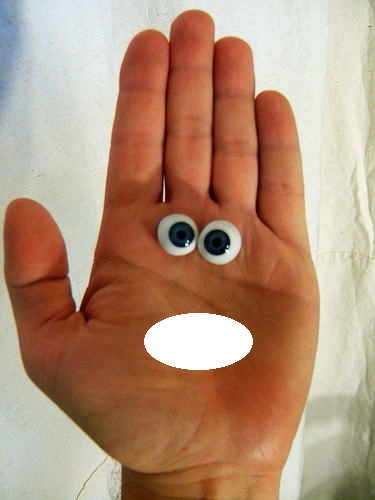
\includegraphics[width=2in]{images/hand.jpg}\label{fig:blend.hand}}
  \hfil
  \subfigure[Second source]{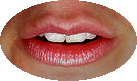
\includegraphics[width=1.23in,trim = -0.5in -1.5in -0.5in 0in]{images/lips.jpg}\label{fig:blend.lips}}
  \hfil
  \subfigure[Blended result]{\includegraphics[width=2in]{images/hand-lips-blend.jpg}\label{fig:blend.result}}
\caption{Example input and output images from the {\tt ImageComposite} multi-band 
blender.\protect\footnotemark }
\label{fig:blend.hand.maincaption}
\end{figure}
\footnotetext{Original hand and face source images by {\tt sheldonschwartz} and {\tt vidrio}, respectively, and released under the Creative Commons license.}

\begin{figure}[p]
\centering
  \subfigure[Draft mode (simple overlay)]{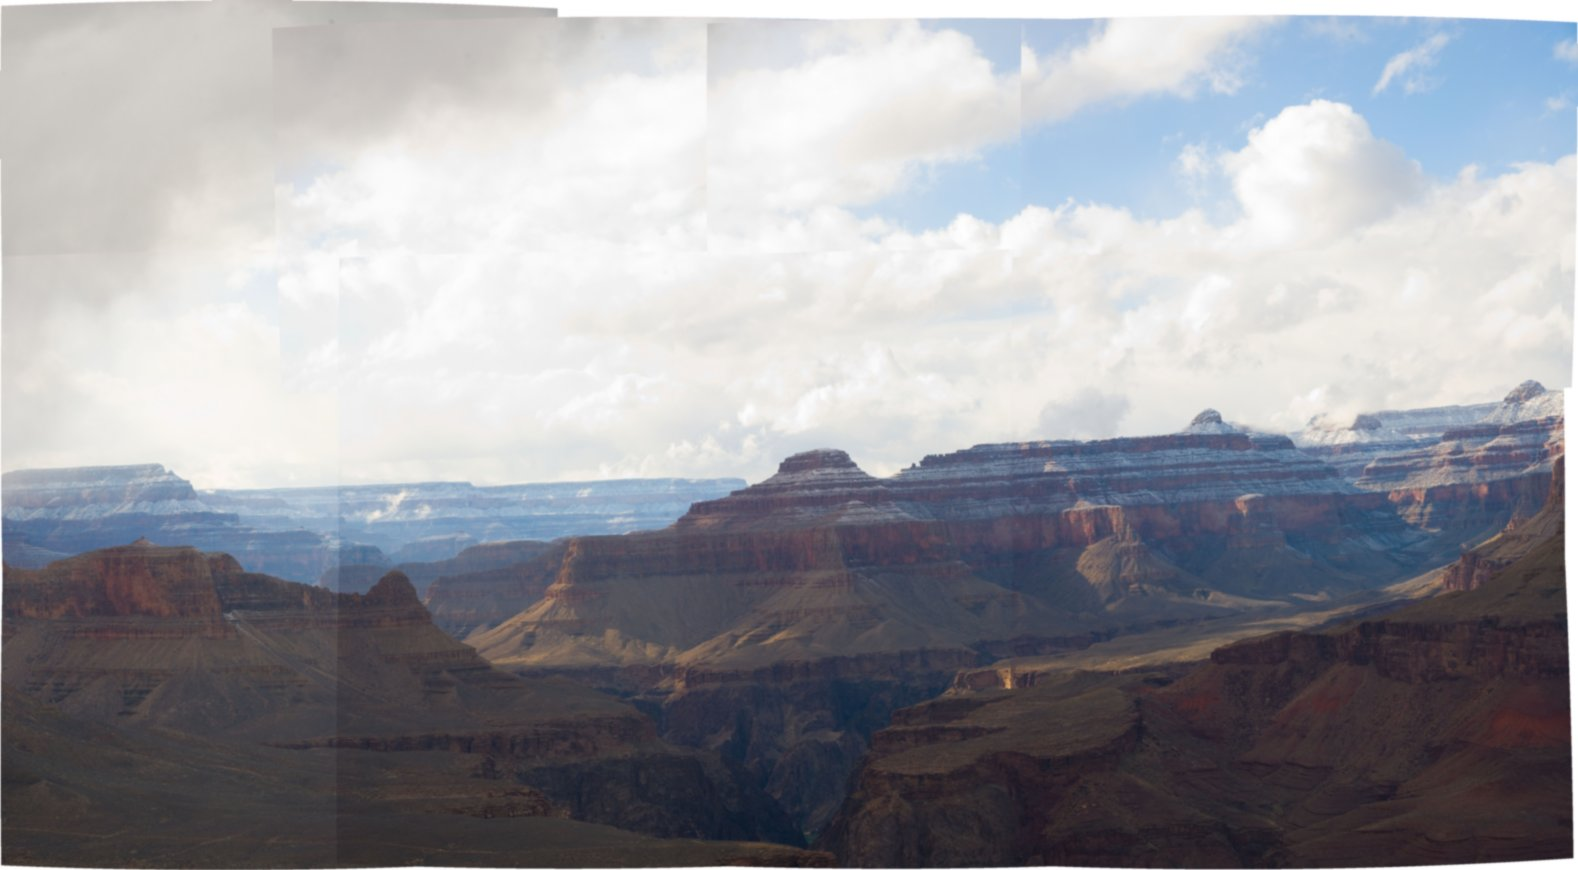
\includegraphics[width=6.5in]{images/kiabab-draft.jpg}\label{fig:kiabab.draft}}
  \\
  \subfigure[Multi-band blending]{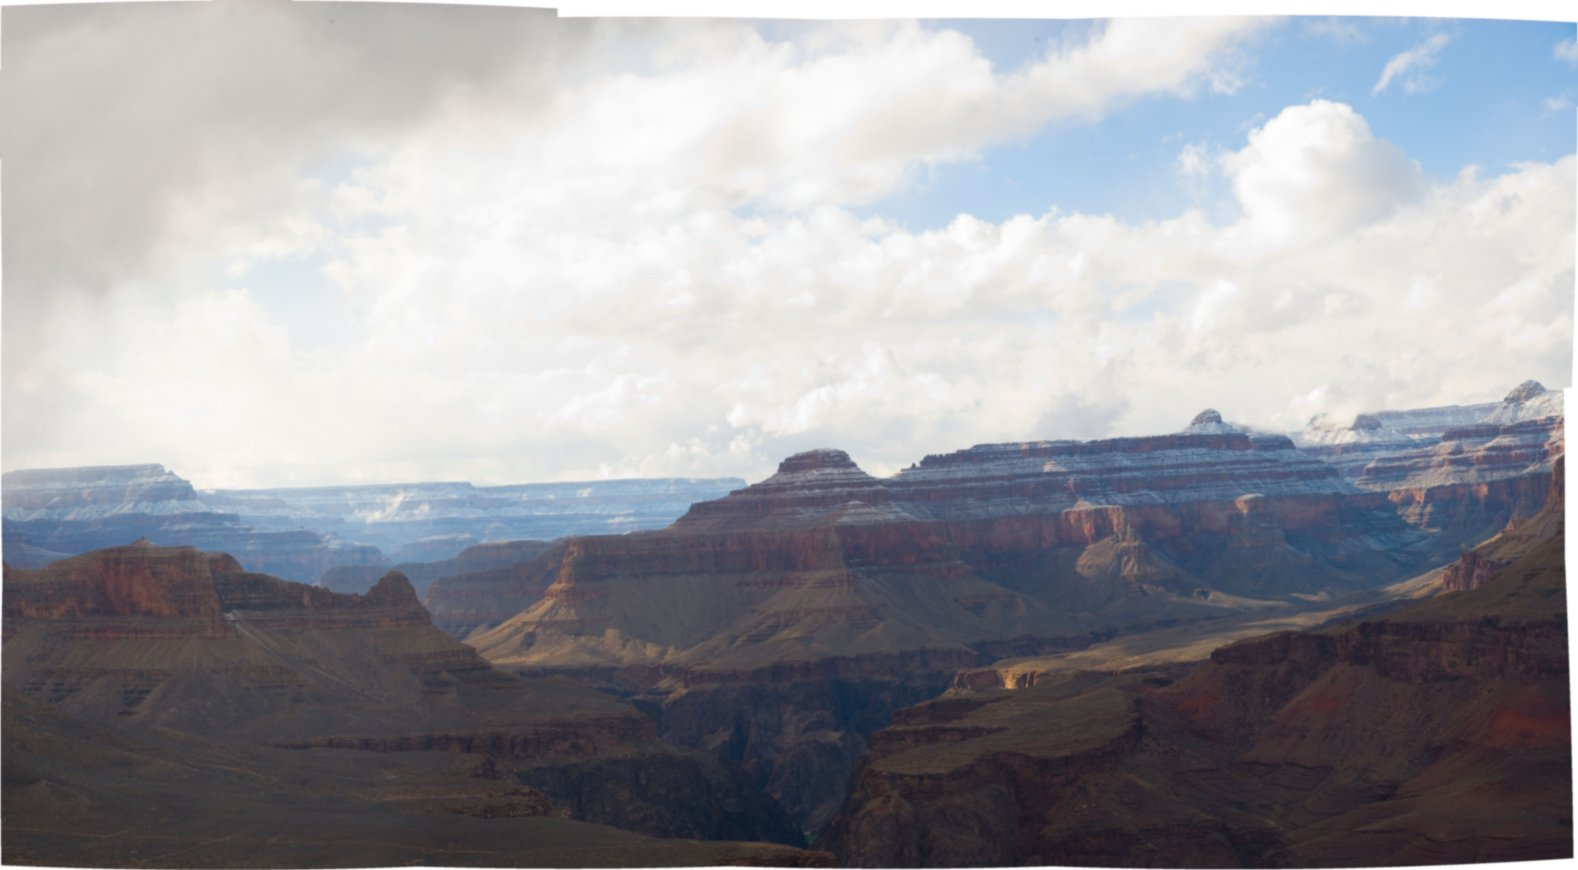
\includegraphics[width=6.5in]{images/kiabab-blend.jpg}\label{fig:kiabab.blend}}
\caption{A twelve-image mosaic composited using an {\tt ImageMosaic} object, first (a) in 
draft mode and then (b) using multi-band blending.}
\label{fig:blend.kiabab}
\end{figure}

\section{{\tt ImageQuadTreeGenerator}}\label{sec:quadtreegenerator}

The ability to assemble composites that are far larger than could be stored 
in memory all at once presents serious challenges.  When viewing an image 
of that size, the ability to zoom in and out is of critical importance.  
Only a small fraction of the image data will ever be on-screen at a time 
at full resolution.  However the entire data set may be visible at once at 
lower resolutions, and computing such reduced images on the fly can be 
prohibitively expensive.  The usual solution to this problem is to 
pre-compute sub-sampled versions of the image at multiple levels of detail. 
The sub-sampling factors are often chosen to be successive powers of two, 
and the data at each resolution is typically chopped up into tiles for 
faster direct access.

The \verb#ImageQuadTreeGenerator# class generates just such a representation 
of an image.  You specify the tile size, the generator reduces the 
image by powers of two until it fits in a single tile.  To generate 
each successive level of detail every tile is replaced by four tiles 
at twice the resolution.  The resulting quad-tree of images is stored 
on disk in a hierarchical manner, making it easy to instantly access any 
tile at any resolution.

Like many things in the Vision Workbench, an \verb#ImageQuadTreeGenerator# 
is templatized on its pixel type.  The constructor takes two arguments, 
the pathname of the tree to be created on disk and the source image. 
You can then use several member functions to configure the quad-tree 
prior to generating it.  The \verb#set_bbox()# method, which takes a 
single \verb#BBox2i# parameter, specifies that a particular region of 
the source image to be processed instead of the entire thing.  The 
\verb#set_output_image_file_type()# method sets the file type of the 
generated image files; the default is ``\verb#png#''.  The 
\verb#set_patch_size()# function takes an integer argument specifying 
the patch size in pixels.  Relatedly, the \verb#set_patch_overlap()# 
function specifies how many pixels of the border of each patch overlap 
the neighboring patch.  The default is $256$-pixel patches with no 
overlap.  Finally, the \verb#set_crop_images()# method takes a 
boolean argument that controls whether or not the resulting images 
are cropped to the non-transparent region.  Image cropping is enabled 
by default.

Once you have configured the \verb#ImageQuadTreeGenerator# to your liking
you can invoke its \verb#generate()# method to generate the quad-tree
on disk.  It is stored in a directory with the name you provided as
the first argument to the constructor with the extension
``\verb#.qtree#'' appended.  For example, if you specified the name of
the quad-tree as \verb#/home/mdh/example# then the result is stored in
the directory \verb#/home/mdh/example.qtree#.  This directory
typically contains three things.  First is the lowest-resolution image
of the tree, essentially a thumbnail, which is stored in an image with
the same base name as the tree with the appropriate image file format 
extension appended.  To continue the above example, if the file format 
type is ``\verb#png#'' then the top-level image file's pathname will be 
\verb#/home/mdh/example.qtree/example.png#.  The next file in the 
top-level directory is a simple text file describing the bounding box 
of the top-level patch, with the same name but with the extension 
\verb#.bbx# instead.  The format of this file will be discussed below.  
Finally there is a subdirectory, which has the same name but no extension,
that contains the next level of the tree.

Inside that subdirectory there are generally four image files, with
names \verb#0.png#, \verb#1.png#, \verb#2.png#, and \verb#3.png#,
containing to the four image patches at the second level of
detail. The patches are numbered left-to-right and top-to-bottom, so
\verb#0# is the upper-left patch, \verb#1# is the upper-right patch,
and so on.  There are also four corresponding \verb#.bbx# files and
four directories containing higher-resolution data for each patch.
Each subdirectory likewise has four numbered images, bounding boxes,
and further subdirectories.  For example, the file
\verb#/foo/bar/myimage.qtree/myimage/0/1/3.png# would be an image at
the fourth level of detail.  The subdirectories at the highest level
of detail have no further subdirectories.  Note that if cropping is
enabled then it is possible that some directories will not have all
four images; this occurs if any of the images is entirely empty.

Each \verb#.bbx# file contains eleven numbers, represented as test
strings, each on a line by itself.  The first is the scale factor of
that tile: it has the value $1$ for the highest-resolution patches and
values of the form $2^n$ for lower-resolution patches.  You can
equivalently think of this number as describing the size of each pixel
at this resolution, as measured in full-resolution pixels.  The next
four numbers describe the bounding box of the patch within the
full-resolution coordinate system.  First are the $x$ and $y$
coordinates of the upper-left pixel, and then come the width and
height of the image in pixels.  To reiterate, these are measured in
{\it full-resolution} pixels, and so these numbers will generally be
multiples of the scale factor.

After this come a similar set of four numbers describing the bounding
box of the unique image data in this patch.  This is generally the
same as the previous bounding box if there is no patch overlap.
However, if the patch overlap has been set to a nonzero value then
this second bounding box will describe the portion of this patch that
does not overlap the corresponding regions of the neighboring patches.
In other words, taken together these second bounding boxes perfectly
tile the entire image without overlap.  Finally, the last two values
describe the width and height of the entire source image in pixels.

This file format is obviously quite arbitrary, and was designed to 
make it easy to write scripts to manipulate the quadtree data later.  
If you prefer, you can subclass the quadtree generator and overload 
the \verb#write_meta_file()# function to generate metadata of a 
different sort.

\begin{figure}[t]
\centering
  \subfigure{\includegraphics[height=1.5in]{images/Walker.qtree/r.jpg}\label{fig:walker.a}}
  \hfil
  \subfigure{\includegraphics[height=1.5in]{images/Walker.qtree/r1.jpg}\label{fig:walker.b}}
  \hfil
  \subfigure{\includegraphics[height=1.5in]{images/Walker.qtree/r12.jpg}\label{fig:walker.c}}
\caption{Patches at three successive resolutions generated by an {\tt ImageQuadTreeGenerator} 
constructed with the name ``{\tt Walker}''.  The files are named {\tt Walker.qtree/Walker.png}, 
{\tt Walker.qtree/Walker/1.png}, and {\tt Walker.qtree/Walker/1/2.png}, respectively.}
\label{fig:blend}
\end{figure}
